%!TEX root =  ./JanasJanssenCuffaro-August2019.tex
%\section{Representing distant correlations by correlation arrays and polytopes} \label{1}

%SUBSECTION 2.1
\subsection{Taking Mermin to Bananaworld} \label{1.1}

The classical tests of Bell's theorem in the 1970s and 1980s were for a version of the Bell inequality formulated by \citet{CHSH}.\footnote{See \citet[Chs.\ 29--31, pp.\ 250--289]{Gilder 2008} for a concise account, written for a general audience and based on interviews with some of the principals, of how the CHSH inequality was formulated and experimentally tested.} The CHSH inequality, like the one originally proposed by \citet{Bell 1964}, is a bound on the strength of distant correlations allowed by local hidden-variable theories. In such theories, the outcomes of the relevant measurements are predetermined by variables not included in the quantum description (hence: hidden) and cannot be affected by signals traveling faster than light (hence: local). The setup used to test the CHSH inequality involves \emph{two parties}, the ubiquitous Alice and Bob, \emph{two settings per party} of some measuring device (e.g., a polarizer or a Dubois magnet as used in a Stern-Gerlach-type experiment), and \emph{two outcomes per setting} (labeled `0' and `1', `$+$' and `$-$', or `up' and `down'). 

\citet[pp.\ 18--19]{Bell 1964} originally considered three rather than four settings, labeled $\{\hat{a}, \hat{b}, \hat{c}\}$. 
In Bell's setup, one party performs measurements using the pair $\{\hat{a}, \hat{b}\}$ while the other uses $\{\hat{b}, \hat{c}\}$. In the CHSH setup the two parties use two pairs that have no setting in common, $\{\hat{a}, \hat{b}\}$ and $\{\hat{a}', \hat{b}'\}$ in our notation. \citet{Mermin 1981, Mermin 1988} kept Bell's three settings but in his setup both parties use all three settings rather than just two of them. He derived a Bell inequality for this setup, so simple that even those without Mermin's pedagogical skills can explain it to a general audience. 

We use the Mermin setup to illustrate the power of some of the tools in \emph{Bananaworld} \citep{Bub 2016}. We represent the correlations Mermin considered by \emph{correlation arrays}, the workhorse of \emph{Bananaworld}, and parametrize these arrays in such a way that they, in turn, can be represented as points in convex sets in so-called \emph{non-signaling cubes}. This approach was pioneered by \citet{Pitowsky 1989b} in \emph{Quantum Probability---Quantum Logic}.\footnote{\citet[p.\ 120]{Bub 2016} also cites \citet{Pitowsky 2006}, his contribution to a \emph{Festschrift} for Bub, as well as \citet{Pitowsky 1986,Pitowsky 1989a,Pitowsky 1991,Pitowsky 2008}.} 

The representation of classes of correlations in terms of convex sets is well-established in the quantum-foundations literature. Our paper can be seen as another attempt to bring this approach to a broader audience by applying it to Mermin's particularly simple and instructive example. The CHSH setup uses four different settings and its non-signaling cube is a hypercube in four dimensions. The Mermin setup only uses three different settings and its non-signaling cube is an ordinary cube in three dimensions, which makes it easy to visualize. The convex set representing the non-signaling correlations allowed classically is a tetrahedron spanned by four of the eight vertices of the non-signaling cube (see Figure \ref{tetrahedron}); the convex set representing those allowed quantum-mechanically is an elliptope enclosing this tetrahedron (see Figure \ref{elliptope}).  

In \emph{Bananaworld}, \emph{settings} become \emph{peelings}, \emph{outcomes} become \emph{tastes}, and \emph{parties} become characters from \emph{Alice in Wonderland} (Alice stars as Alice, the White Rabbit as Bob). Bananas can be peeled ``from the stem end ($S$)'' or ``from the top end ($T$)'' and can only taste ``\emph{o}rdinary (``o'' or 0)'' or ``\emph{i}ntense, \emph{i}ncredible,  \emph{i}ncredibly delicious (``i'' or 1)'' \citep[pp.\ 8--9, see also p.\ viii]{Bub 2016}.\footnote{Betraying his information-theoretic leanings, \citet{Bub 2016} occasionally refers to \emph{inputs} and \emph{outputs} (both taking on the values 0 and 1) rather than peelings and tastes (see, e.g., p.\ 51, Figure 3.1).} Bub's banana-peeling scheme suffices for the discussion of the CHSH inequality as well as for the analysis of PR boxes, at least those of the original design of their inventors,  \citet{Popescu and Rohrlich 1994}. A PR box is a hypothetical system allowing \emph{superquantum correlations} \citep[p.\ 106]{Bub 2016}, non-signaling correlations that are stronger 
(in some sense to be explicated later)
%(by measures to be introduced below) 
than those allowed by quantum mechanics. Like the CHSH setup, the original design of a PR box involved two parties, two settings per party, and two outcomes per setting. Bub's scheme also works for the analysis of correlations that arise in measurements on so-called GHZ states \citep{GHZ}. While these measurements involve three rather than two parties,\footnote{Bub's illustrator, his daughter Tanya, has the Cheshire Cat (starring as Clio) peel the third GHZ banana \citep[pp.\ 122--123, Clio and Charlie are introduced on p.\ 8]{Bub 2016}.} they still fit the mold of two settings per party and two outcomes per setting. The Mermin setup breaks this mold by using (the same) three settings for both parties. 

To recreate the Mermin setup in \emph{Bananaworld} we thus need a new banana-peeling scheme. Our scheme not only allows infinitely many different settings, it also highlights elements of spherical symmetry in the setups we will examine that turn out to be key to their quantum-mechanical analysis (see Section \ref{2.1}). Figures \ref{AliceBob-Mermin}--\ref{AliceBob-tasting} illustrate our \emph{Bananaworld} version of the Mermin setup.  

\begin{figure}[ht]
\centering
    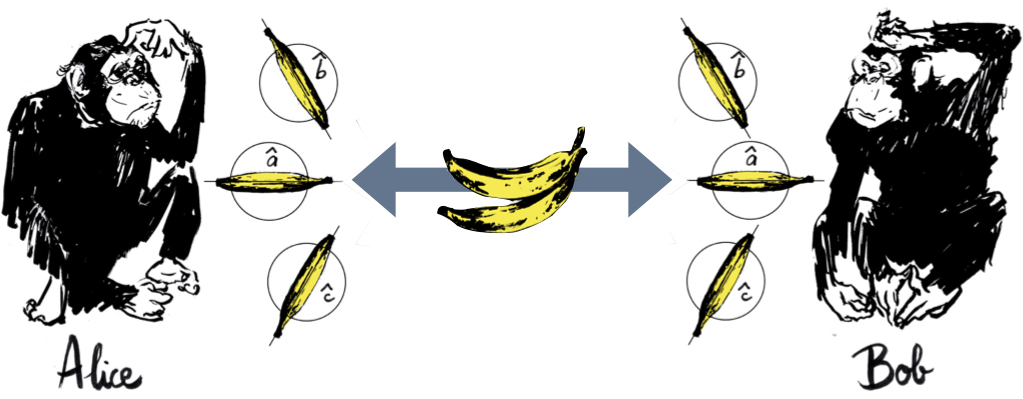
\includegraphics[width=4.5in]{AliceBob-Mermin.jpg}
 \caption{Taking Mermin to \emph{Bananaworld} (I). \emph{Two parties}: the \emph{chimps} Alice and Bob. \emph{Three settings per party}: three \emph{peelings}, ($\hat{a}, \hat{b}, \hat{c}$), given by three unit vectors $(\vec{e}_a, \vec{e}_b, \vec{e}_c)$, in the corresponding \emph{peeling directions} (i.e., the direction of the line going from the top to the stem of the banana while it is being peeled). In Mermin's example, the angles $\varphi_{ab}$ between $\vec{e}_a$ and $\vec{e}_b$, $\varphi_{ac}$ between $\vec{e}_a$ and $\vec{e}_c$, and $\varphi_{bc}$ between $\vec{e}_b$ and $\vec{e}_c$ are all equal to $120\degree$. Drawing by Laurent  Taudin with a nod to Andy Warhol.}
 %(see note \ref{warhol})}
   \label{AliceBob-Mermin}
\end{figure}

We focus on a species of banana that grows in pairs on special banana trees. These bananas can only taste yummy or nasty. Yet we cannot say that they come in two flavors, as they only acquire a definite flavor once they are peeled and tasted. We use these bananas in a long series of peel-and-taste experiments following a protocol familiar from experimental tests of Bell inequalities. We pick a pair of bananas, still joined at the stem, from the banana tree. We separate them and give one each to two chimps, Alice and Bob. Once they have received their respective bananas, they randomly and independently of one another pick a particular \emph{peeling}, defined by the \emph{peeling direction}, i.e., the direction of the line going from the top to the stem of the banana while it is being peeled. Alice and Bob are instructed not to change the orientation of their bananas while peeling so that it is unambiguous which peeling they are using. In the Mermin setup, Alice and Bob get to choose between three peelings, labeled $\hat{a}$, $\hat{b}$ and $\hat{c}$, represented by unit vectors, $\vec{e}_a$, $\vec{e}_b$ and $\vec{e}_c$, in the corresponding peeling directions (see Figure \ref{AliceBob-Mermin}). Once they have randomly chosen one of these three peelings, they point the stem of their banana in the direction of the corresponding unit vector and peel their banana (it does not matter whether they peel from the top or from the stem). When done peeling, Alice and Bob reposition their bananas and take a bite to determine whether they taste yummy or nasty (see Figure \ref{AliceBob-tasting}). The whole procedure is then repeated with a fresh pair of bananas from the banana tree. 

\begin{figure}[ht]
\centering
    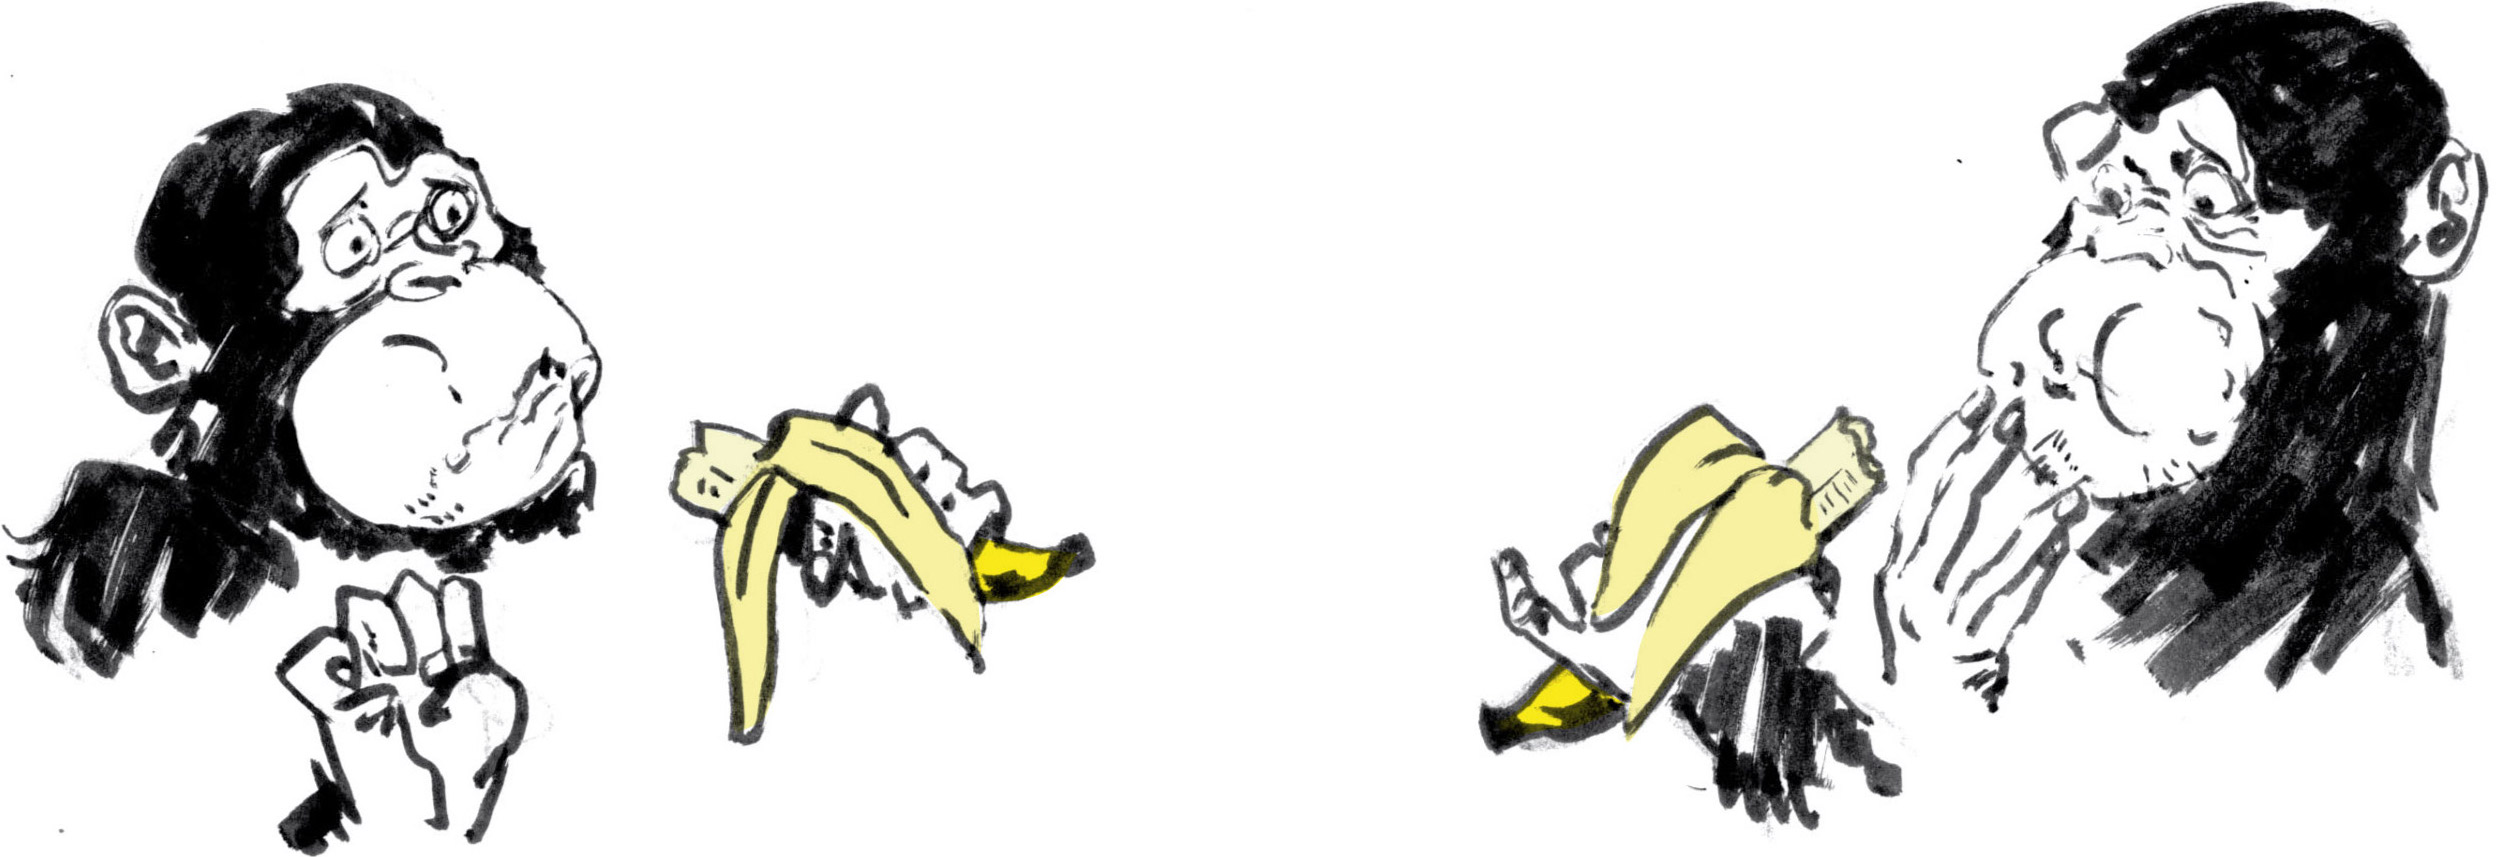
\includegraphics[width=4.5in]{AliceBob-tasting.jpg}
 \caption{Taking Mermin to \emph{Bananaworld} (II). \emph{Two outcomes per setting}: the \emph{tastes} ``yummy'' ($+$) or ``nasty'' ($-$) for different peeling directions. The peeling and tasting is done by the chimps Alice and Bob. Drawing by Laurent Taudin.}
   \label{AliceBob-tasting}
\end{figure}

In each run of this peel-and-taste experiment, Alice and Bob record that run's ordinal number, the peeling chosen ($\hat{a}$, $\hat{b}$ or $\hat{c}$) and the taste of their banana, using ``$+$'' for ``yummy'' and ``$-$'' for ``nasty''. Every precaution is taken to ensure that, as long as there are more bananas to be peeled and tasted, Alice and Bob cannot communicate. While they are peeling and tasting, the only contact between them is that the bananas they are given come from pairs originally joined at the stem on the banana tree.

When all bananas are peeled and tasted, Alice and Bob are allowed to compare notes. Just looking at their own records, they see nothing out of the ordinary---just a sequence of pluses and minuses as random as if they had faked their results by tossing a coin for every run. Comparing their records, however, they note that, every time they happened to choose the same peeling (in roughly $33 \%$ of the total number of runs), their results are perfectly anti-correlated. Whenever one banana tasted yummy, its twin tasted nasty. In and of itself, this is not particularly puzzling. Maybe our bananas always grow in pairs in which one is predetermined to taste yummy while its twin is predetermined to taste nasty. This simple explanation, however, is ruled out by another striking correlation our chimps discover while pouring over their data. When they happened to peel differently (in roughly $66 \%$ of the runs), their results were positively correlated, albeit imperfectly. In 75\% of the runs in which they used different peelings, their bananas tasted the same \citep[p.\ 86]{Mermin 1981}.\footnote{In Mermin's (1981, p.\ 86) example, there is a perfect (positive) correlation in runs in which the two parties use the same setting and an imperfect anti-correlation in runs in which they use different settings (see also Mermin, 1988, pp.\ 135--136). To get Mermin's original example, we should have used our pairs of bananas to represent entangled pairs of photons and let ``peel and taste bananas using different peeling directions'' stand for ``measure the polarization of these photons along different axes''. We got our variation on Mermin's example by having pairs of bananas represent pairs of spin-$\frac12$ particles entangled in the singlet state and letting ``peel and taste bananas using different peeling directions''  stand for ``measure spin components of these particles along different axes'' (see Section \ref{1.5}).\label{mermin}} The tastes of two bananas coming from one pair thus depend on the angle between the peeling directions used. This is certainly odd but one could still imagine that our bananas are somehow pre-programmed to respond differently to different peelings and that the set of pre-programmed responses is different for the two bananas in one pair. What Mermin's Bell inequality shows, however, is that it is impossible to pre-program twin bananas in such a way that they would produce the specific correlations found in this case. Such correlations, however, can and have been produced with quantum twins (see Section \ref{1.5}). Given that they persist no matter how far we imagine Alice and Bob to be apart, another explanation of these curious correlations is also unavailing: it would take a signal traveling faster than the speed of light for the taste of one banana peeled a certain way to either affect the way the other banana is peeled or affect its taste when peeled that way. In short, these correlations cannot be accounted for on the basis of any local hidden-variable theory. 

%SUBSECTION 2.2
\subsection{Non-signaling correlation arrays} \label{1.2}

The correlations found in the Mermin setup can be represented in a correlation array consisting of nine cells, one for each of the nine possible combinations of peelings (see Figure \ref{CA-3set2out-Mermin} in Section \ref{1.3}). These cells form a grid with three rows for Alice's three peeling directions and three columns for Bob's. Each cell has four entries, giving the probabilities of the four possible pairs of tastes for that cell's combination of peelings (the entries in one cell thus always sum to 1). 

Since \emph{Bananaworld} focuses on setups with two settings per party, all correlation arrays in it have only four cells. These cells form a $2 \times 2$ grid with rows for Alice peeling from the stem and from the top and columns for Bob peeling from the stem and from the top. Before we turn to the $3 \times 3$ Mermin correlation array we go over some properties of these simpler $2 \times 2$ correlation arrays. 

\begin{figure}[ht]
 \centering
   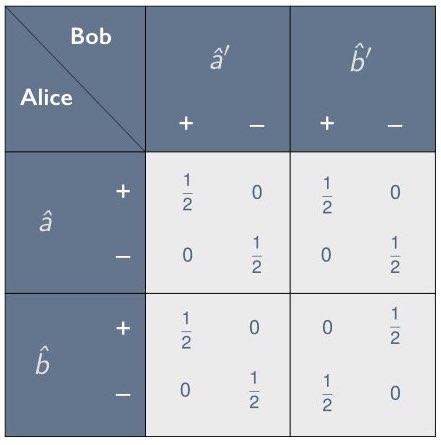
\includegraphics[width=2.5in]{CA-PRbox.jpeg} 
   \caption{Correlation array for a Popescu-Rohrlich box.}
   \label{CA-PRbox}
\end{figure}  

The correlation array  in Figure \ref{CA-PRbox} for a PR box in its original design is an example of such an array \citep[p.\ 89, Table 4.2; we switched Alice and Bob to match the convention that the index labeling the rows of a matrix comes before the index labeling its columns]{Bub 2016}. This correlation array plays an important role in \emph{Bananaworld} and is central to its sequel, Tanya and Jeffrey Bub's (2018) enchanting \emph{Totally Random}. A version of it is prominently displayed on many pages of this graphic novel \citep[pp.\ 15, 21, 33, 95, 115, 181, 200 and 227]{Bub and Bub 2018}. The version in \emph{Totally Random} differs in two respects from the version in Figure \ref{CA-PRbox} (which follows \emph{Bananaworld}). First, in Figure \ref{CA-PRbox}, the outcomes found by Alice and Bob are perfectly correlated in three of the four cells, while they are perfectly anti-correlated in the remaining one. In \emph{Totally Random} it is just the other way around. Second, instead of the four entries in each cell in Figure \ref{CA-PRbox}, the cells in \emph{Totally Random} just have ``$=$'' for perfectly correlated and ``$\neq$'' for perfectly anti-correlated. 

In \emph{Bananaworld} the PR-box correlations in Figure \ref{CA-PRbox} are realized with the help of PR bananas growing in pairs on PR banana trees. The settings $\{\hat{a}, \hat{b}\}$ and $\{\hat{a}', \hat{b}'\}$ now stand for Alice and Bob peeling their bananas from the stem ($S$) or from the top ($T$). These peelings could be replaced by two of the peeling directions we introduced. In realizations of this PR box, we can (but do not have to) use the same pair of settings for Alice and Bob (in the case of the CHSH setup we definitely need different pairs of settings; see Section \ref{3}).  

In \emph{Totally Random}, the PR-box correlations  in Figure \ref{CA-PRbox}  are realized with the help of an imaginary device, named for the inventors of the PR box, the ``Superquantum Entangler PR01''. This gadget, which looks like a toaster, has slots for two US quarters. When we insert two ordinary coins, the PR01 turns them into a pair of entangled ``quoins'' \citep[p.\ 7]{Bub and Bub 2018}. The different settings now stand for Alice and Bob holding their quoins heads-up ($\hat{a} = \hat{a}'$) or tails-up ($\hat{b} = \hat{b}'$) when tossing them. The outcomes are the quoins landing heads or tails. What makes this a realization of a PR box with the correlation array shown in Figure \ref{CA-PRbox} is that the quoins invariably land with the same side facing up, except when both are tossed being held tails-up ($\hat{b}, \hat{b}'$), in which case they always land with opposite sides facing up. 

The correlations between the outcomes found in a PR box---be it between the tastes of a pair of PR bananas or the landings of a pair of quoins---are preserved no matter how far its two parts are pulled apart.\footnote{Part of what makes it interesting to contemplate entangled quoins or bananas is that we are free to choose \emph{when} to toss or taste them whereas with entangled photons or spin-$\frac12$ particles we have no choice but to measure their polarization or spin as soon as they arrive at our detectors.} 

An important feature of correlation arrays (no matter how many cells they have or how many entries each cell has) is that they allow us to see at a glance whether or not the correlations they represent can be used for the purposes of instant messaging or superluminal signaling. Suppose Alice wants to use the peeling of a pair of PR bananas to instant-message the answer to some ``yes/no'' question to Bob. They agree ahead of time that Alice will peel $\hat{a}$ if the answer is ``yes'' and $\hat{b}$ if it is ``no''.\footnote{It does not matter in what order Alice and Bob peel their bananas. The correlations in the correlation array in Figure \ref{CA-PRbox} represent constraints on possible combinations of outcomes found by Alice and Bob, not some mechanism through which the outcome of one peeling would cause the outcome of the other.\label{peeling order irrelevant}}  This scheme will not work. No matter how Bob peels his banana, he cannot tell from its taste whether Alice peeled hers $\hat{a}$ or $\hat{b}$. Suppose Bob peels $\hat{b}'$ (essentially the same argument works if Bob peels $\hat{a}'$). In that case, the correlation array in Figure \ref{CA-PRbox} tells us that the marginal probability of Bob finding $+$  if Alice were to peel $\hat{a}$ (trying to transmit ``yes'') is
\begin{equation}
\mathrm{Pr}(+_{\mathrm B}| \hat{a} \,\hat{b}') = \mathrm{Pr}(+\!+| \hat{a} \,\hat{b}') \, + \, \mathrm{Pr}(-\!+| \hat{a} \,\hat{b}') =  \sfrac12 + 0 = \sfrac12,
\label{non-signaling property 1}
\end{equation}
which is the same as the marginal probability of him finding $+$  if Alice were to peel $\hat{b}$ (trying to transmit ``no''):
\begin{equation}
\mathrm{Pr}(+_{\mathrm B}| \hat{b} \,\hat{b}') = \mathrm{Pr}(+\!+| \hat{b} \,\hat{b}') \; + \; \mathrm{Pr}(-\!+| \hat{b} \,\hat{b}') =  0 + \sfrac12 = \sfrac12.
\label{non-signaling property 2}
\end{equation}
Inspection of the correlation array in Figure \ref{CA-PRbox} shows that \emph{all} such marginal probabilities are equal to $\sfrac12$ in this case. PR boxes---whether realized with the help of magic bananas, quoins, or other systems---cannot be used for instant messaging. 

Correlations that do not allow instant messaging are called \emph{non-signaling}. It will be convenient to use this term for their correlation arrays as well. The correlations and correlation arrays for a PR box are always non-signaling. In fact, this is what makes these hypothetical devices intriguing. Even though they would give rise to correlations stronger than those allowed by quantum mechanics, they would not violate special relativity's injunction against superluminal signaling.

Generalizing the results in Eqs.\ (\ref{non-signaling property 1})--(\ref{non-signaling property 2}), we can state the following \emph{non-signaling condition}:
\begin{quote}
\emph{A correlation in a setup with two parties, two settings per party and two outcomes per setting is \emph{non-signaling} if the probabilities in both rows and both columns of all cells in its correlation array add up to $\sfrac12$.}
\end{quote}
The converse is not true. A correlation array with the entries
\begin{equation}
\begin{array}{cccc}
1  & 0  & 0 & 1 \\[.1 cm]
 0 & 0  & 0 & 0 \\[.1 cm]
 0 & 0  & 0 & 0 \\[.1 cm]
1 & 0 & 0 & 1
\end{array}
\end{equation}
is non-signaling even though the entries in half the rows and columns of its cells add up to 1 while the entries in the other half add up to 0. The relevant marginal probabilities, however, are still equal to each other. For instance,
\begin{equation}
\mathrm{Pr}(+_{\mathrm B}|\hat{a} \,\hat{b}') = \mathrm{Pr}(+_{\mathrm B}|\hat{b} \,\hat{b}') = 0 \quad \mathrm{ and} \quad \mathrm{Pr}(-_{\mathrm B}|\hat{a} \,\hat{b}') = \mathrm{Pr}(-_{\mathrm B}|\hat{b} \,\hat{b}') = 1.
\end{equation}
In Section \ref{2}, we will encounter correlation arrays for setups with three outcomes per setting that are non-signaling even though not all rows and columns of its cells add up to the same number (see Figure \ref{CA-3set3out-raffle-vi} in Section \ref{2.2.2}).\footnote{In \emph{Bananaworld}, Bub leaves it to the reader to find examples of correlation arrays that violate the non-signaling condition. Below are the entries for two such correlation arrays:
$$
(a) \quad \begin{array}{cccc}
1  & 0  & 0 & 0 \; \\
 0 & 0  & 0 & 1 \; \\
 0 & 0  & 1 & 0 \; \\
 0 & 1 & 0 & 0,
\end{array}
\quad \quad \quad
(b) \quad \begin{array}{cccc}
\boldsymbol{6/10}  & 1/10  & 2/10 & 1/10 \; \\
1/10  & 2/10  & 1/10 & \boldsymbol{6/10} \; \\
2/10  & 1/10  & \boldsymbol{6/10} & 1/10 \; \\
1/10  & \boldsymbol{6/10}  & 1/10 & 2/10.
\end{array}
$$
If there were a system producing the distant correlations in (a), be it pairs of bananas or pairs of coins, one pair would suffice for Alice and Bob to transmit one bit of information to the other party instantaneously; if there were a system producing the distant correlations in (b), several pairs would be needed to do so with some fidelity. The latter system can be thought of as a noisy version of the former.}

%SUBSECTION 2.3
\subsection{Non-signaling cubes, classical polytopes and the elliptope} \label{1.3}

Any cell in a non-signaling correlation array for any number of settings with two outcomes per setting can be parametrized by a variable with values running from $-1$ to $+1$. Figure  \ref{CA-2set2out-cell} shows such a cell for Alice using setting $\hat{a}$ and Bob using setting $\hat{b}$. Let $-1 \ge \chi_{ab} \ge 1$ be the variable parametrizing this cell. If $\chi_{ab} = 0$, the results of Alice and Bob are uncorrelated; if $\chi_{ab} =-1$, they are perfectly correlated; if $\chi_{ab} =1$, they are perfectly anti-correlated. We will thus call $\chi_{ab}$ an \emph{anti-correlation coefficient.}
\begin{figure}[ht]
\centering
    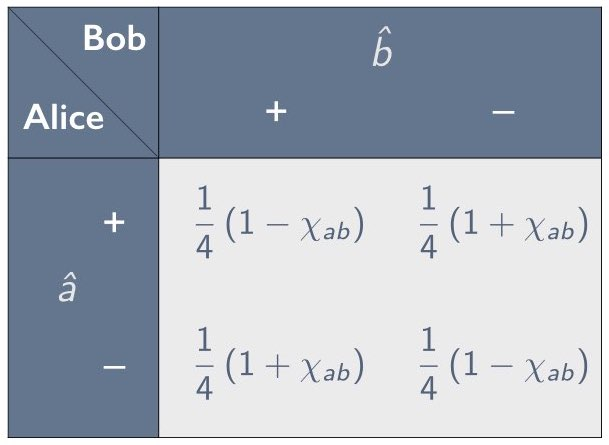
\includegraphics[width=3in]{CA-2set2out-cell.jpeg}
 \caption{Cell in a non-signaling correlation array parametrized by $-1 \le \chi_{ab} \le 1$.}
   \label{CA-2set2out-cell}
\end{figure}

Consider the random variable $X_a^A$ measured by Alice using setting $\hat{a}$ and the random variable $X_b^B$ measured by Bob using setting $\hat{b}$. The  \emph{covariance} of these two variables is defined as the expectation value of the product of $X_a^A - \langle X_a^A \rangle$ and $X_b^B - \langle X_b^B \rangle$, where $\langle X \rangle$ is the expectation value of $X$:
\begin{equation}
\mathrm{cov} \! \left( X_a^A, X_b^B \right) \equiv \left\langle \left( X_a^A - \langle X_a^A \rangle \right) \left( X_b^B - \langle X_b^B \rangle \right) \right\rangle.
\label{cov def 0}
\end{equation}
The random variables we will be considering are all \emph{balanced}. That a random variable is \emph{balanced} means that it has the following two properties:
\begin{quote}
A random variable $X$ is balanced IFF
\begin{equation}
\begin{array}{l}
\text{(1) if $x$ is a possible value, then $-x$ is a possible value as well;} \\[.2cm]
\text{(2) the value $x$ is as likely to occur as the value $-x$.} 
\end{array}
\label{def balanced}
\end{equation}
\end{quote}
Such variables have zero expectation value, which means that Eq.\ (\ref{cov def 0}) reduces to:
\begin{equation}
\mathrm{cov} \! \left( X_a^A, X_b^B \right) = \left\langle  X_a^A \, X_b^B \right\rangle.
\label{cov def}
\end{equation}
Bell inequalities (including the CHSH one) are typically expressed in terms of such expectation values. To compute $\langle  X_a^A \, X_b^B \rangle$, we need to assign a numerical value to the taste of a banana. To this end, we introduce the \emph{Bub} or \emph{banana constant} $b$. Yummy ($+$) and nasty ($-$) then correspond to $\pm \bbar/2$, where $\bbar \equiv b/2\pi$ (called \emph{banana split} or \emph{banana bar}). Using the entries in the correlation array in Figure \ref{CA-2set2out-cell}, we evaluate the expectation value of the product of $X_a^A$ and $X_b^B$:
\begin{eqnarray}
\bigl\langle X_a^A \, X_b^B \bigr\rangle & = & \frac{\bbar^2}{4} \biggl(\mathrm{Pr}(+\!+| \hat{a} \,\hat{b})
 \mathrm{Pr}(-\!-| \hat{a} \,\hat{b})\biggr) \nonumber\\
&& - \frac{\bbar^2}{4} \biggl(\mathrm{Pr}(+\!-| \hat{a} \,\hat{b}) \, + \, \mathrm{Pr}(-\!+| \hat{a} \,\hat{b})\biggr) \nonumber \\
& =  &\frac{\bbar^2}{4} \biggl( \frac12 (1 - \chi_{ab}) - \frac12 (1 + \chi_{ab}) \biggr) \; = \; -\frac{\bbar^2}{4} \chi_{ab}.
\label{prob 2 exp}
\end{eqnarray}
Introducing the standard deviations of $X_a^A$ and $X_b^B$,
\begin{equation}
\begin{array}{c}
\sigma^A_a \equiv \sqrt{ \left\langle (X^A_a)^2 - \langle X_a^A \rangle^2 \right\rangle} = \sqrt{ \left\langle (X^A_a)^2 \right\rangle }= \displaystyle{\frac{\bbar}{2}},    \\[.4cm]
\sigma^B_b \equiv  \sqrt{ \left\langle (X^B_b)^2 - \langle X_b^B \rangle^2 \right\rangle} = \sqrt{ \left\langle (X^B_b)^2 \right\rangle }= \displaystyle{\frac{\bbar}{2}}  
\end{array}
\label{standard deviations a and b}
\end{equation}
where we used that $\langle X_a^A \rangle = \langle X_b^B \rangle = 0$, we can thus write the parameter $\chi_{ab}$  introduced in Figure \ref{CA-2set2out-cell} as
\begin{equation}
\chi_{ab} = - \frac{\left\langle X_a^A \, X_b^B \right\rangle}{\sigma^A_a \sigma^B_b}. 
\label{chi as corr coef}
\end{equation}
This is our formal justification for calling $\chi_{ab}$ (and parameters like it for other cells in this and other correlation arrays) an \emph{anti-correlation coefficient}: it is \emph{minus} what is commonly known as \emph{Pearson's correlation coefficient}. We will return to this information-theoretic interpretation of $\chi_{ab}$ in Section  \ref{1.6}.

\begin{figure}[ht]
\centering
    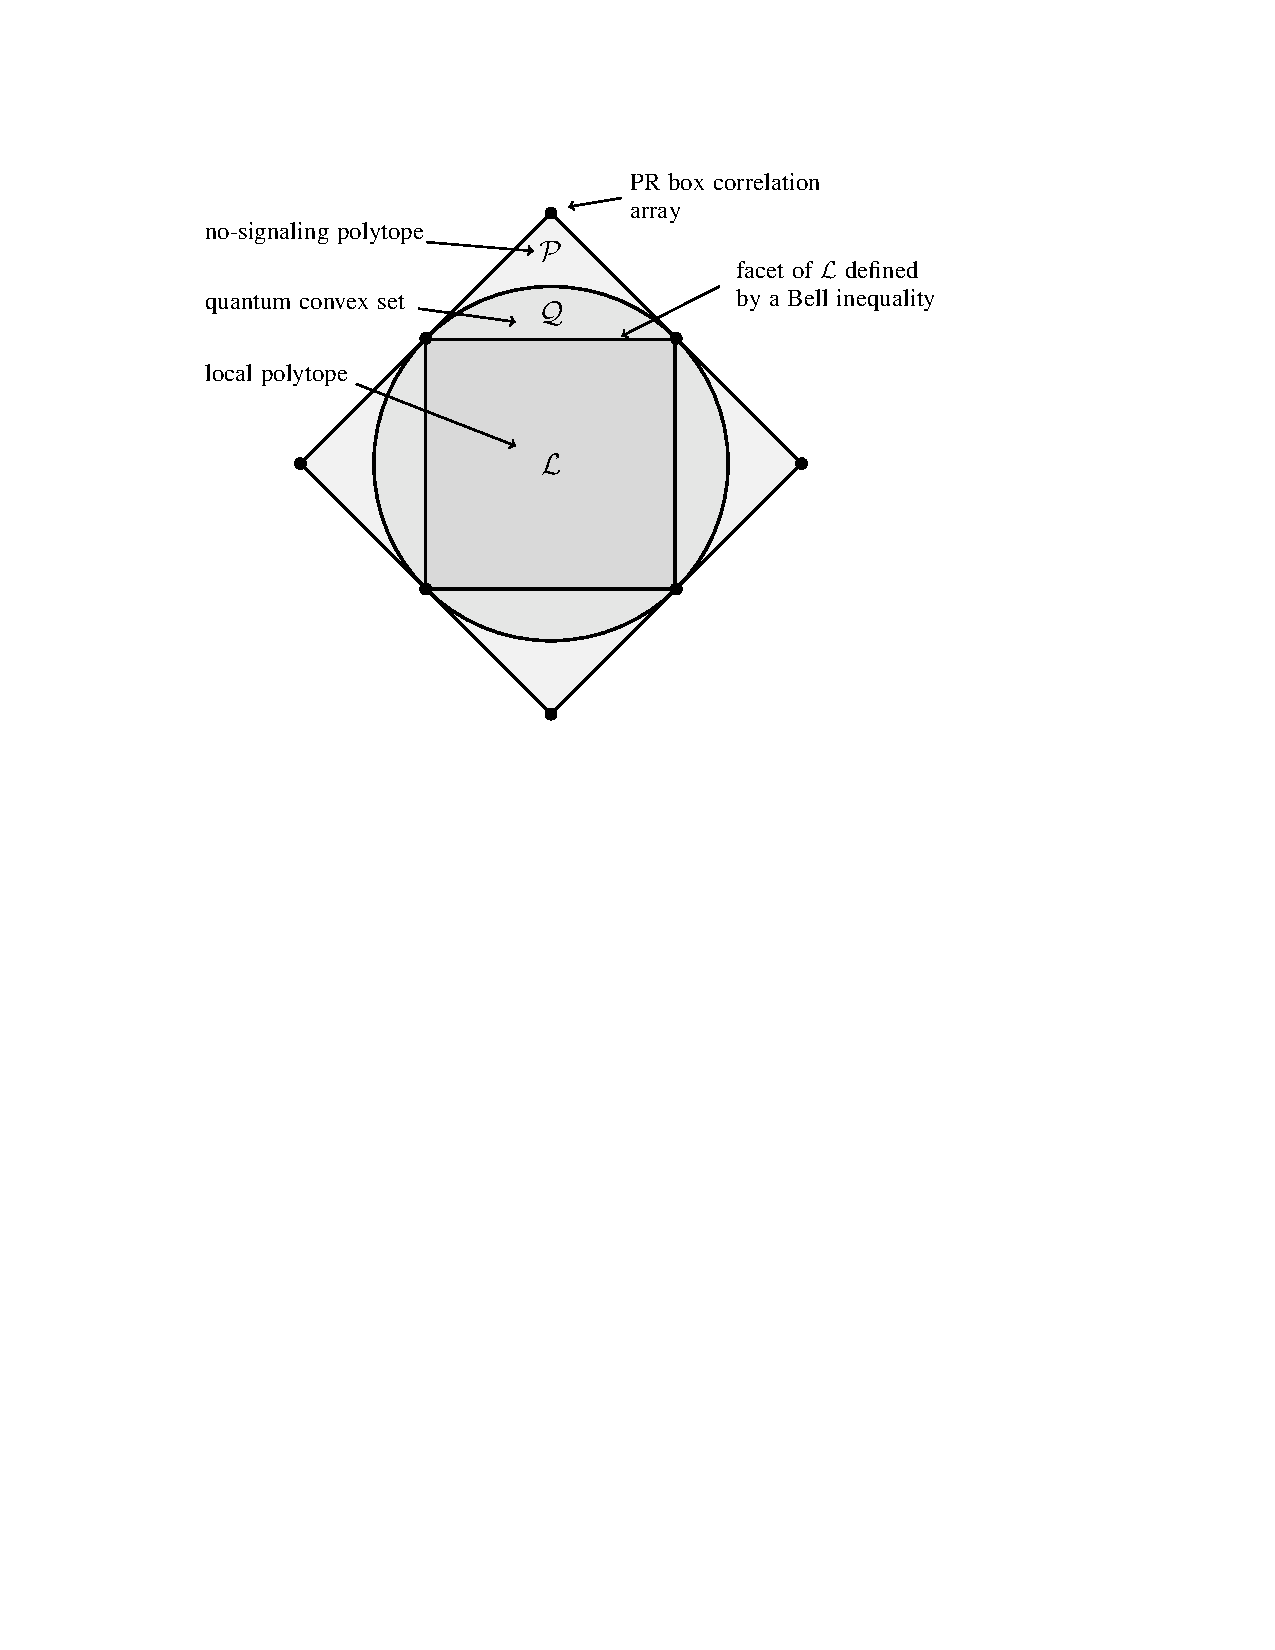
\includegraphics[width=4.5in]{LQP.pdf}
 \caption{A schematic representation, for some arbitrary experimental setup, of the set $\mathcal{P}$ of all non-signaling correlations, the subset $\mathcal{Q} \subset \mathcal{P}$ of those allowed quantum-mechanically and the subset $\mathcal{L} \subset \mathcal{Q}$ of those allowed classically. One of the facets of $\mathcal{L}$ represents a Bell inequality. The vertex of the non-signaling cube where this Bell inequality is maximally violated represents a PR box for the setup under consideration \citep[p.\ 107, Figure 5.2]{Bub 2016}.}
   \label{LQP}
\end{figure}

A $2 \times 2$ non-signaling correlation array such as the one in Figure \ref{CA-PRbox} for a PR box, with four cells of the form of Figure \ref{CA-2set2out-cell}, can be parametrized by four anti-correlation coefficients
\begin{equation}
-1 \le \chi_{aa'} \le 1, \quad -1 \le \chi_{ab'} \le 1, \quad -1 \le \chi_{ba'} \le 1, \quad -1 \le \chi_{bb'} \le 1.
\label{chi values for PR box}
\end{equation}
Such a correlation array can thus be represented by a point in a hypercube in four dimensions with the anti-correlation coefficients serving as that point's Cartesian coordinates. The correlation array for a PR box is represented by one of the vertices of this hypercube: 
\begin{equation}
(\chi_{aa'}, \chi_{ab'}, \chi_{ba'}, \chi_{bb'}) = (-1, -1, -1, 1).
\label{PR box vertices}
\end{equation}
The four-dimensional hypercube that represents the class of all non-signaling correlations in this setup (two parties, two settings per party, two outcomes per setting) is an example of a so-called \emph{non-signaling polytope}, which can be defined (typically in some higher-dimensional space) for setups with two parties, any number of settings and any number of outcomes per setting. 

\begin{figure}[ht]
 \centering
   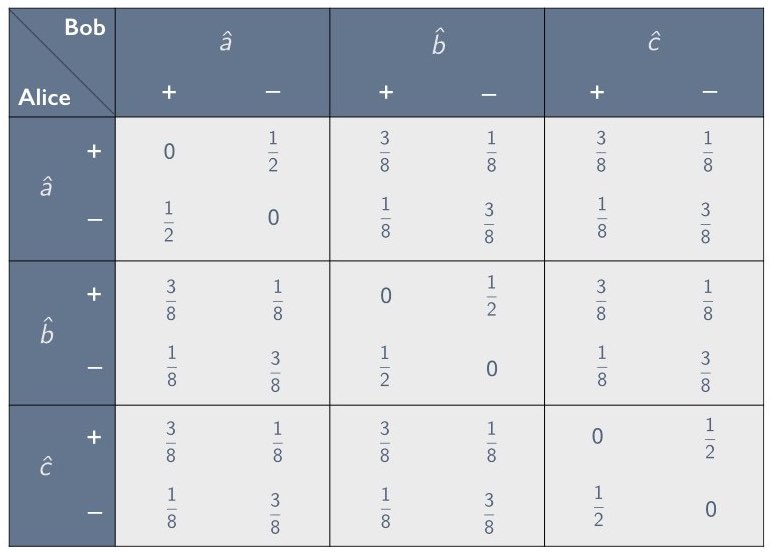
\includegraphics[width=4.5in]{CA-3set2out-Mermin.jpeg} 
   \caption{Correlation array for the correlations found in our variation of the Mermin setup (see Figures \ref{AliceBob-Mermin} and \ref{AliceBob-tasting} and note \ref{mermin}).}
   \label{CA-3set2out-Mermin}
\end{figure}

\begin{figure}[ht]
 \centering
   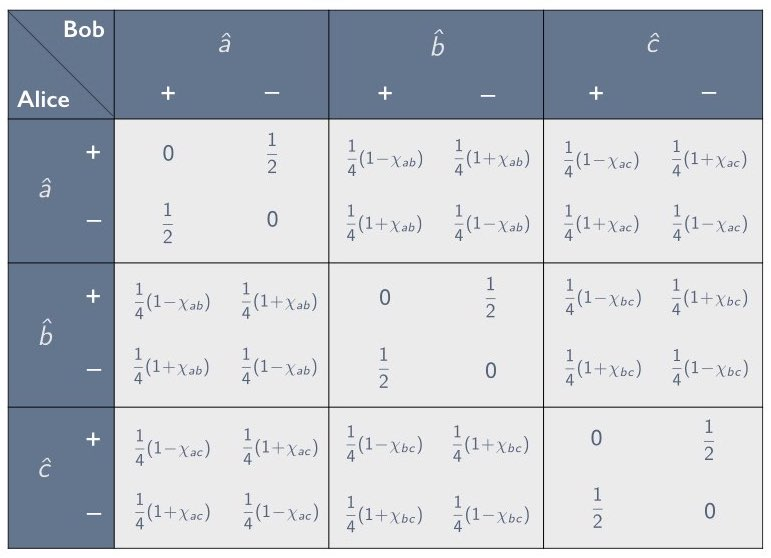
\includegraphics[width=4.5in]{CA-3set2out-non-signaling-chis.jpeg} 
   \caption{A non-signaling correlation array for three settings (peelings) and two outcomes (tastes) parametrized by the anti-correlation coefficients $-1 \le \chi_{ab} \le 1$ (for the $\hat{a} \, \hat{b}$ and  $\hat{b} \, \hat{a}$ cells), $-1 \le \chi_{ac} \le 1$ (for the $\hat{a} \, \hat{c}$ and  $\hat{c} \, \hat{a}$ cells) and $-1 \le \chi_{bc} \le 1$ (for the $\hat{b} \, \hat{c}$ and  $\hat{c} \, \hat{b}$ cells).}
   \label{CA-3set2out-non-signaling-chis}
\end{figure}

\begin{figure}[ht]
\centering
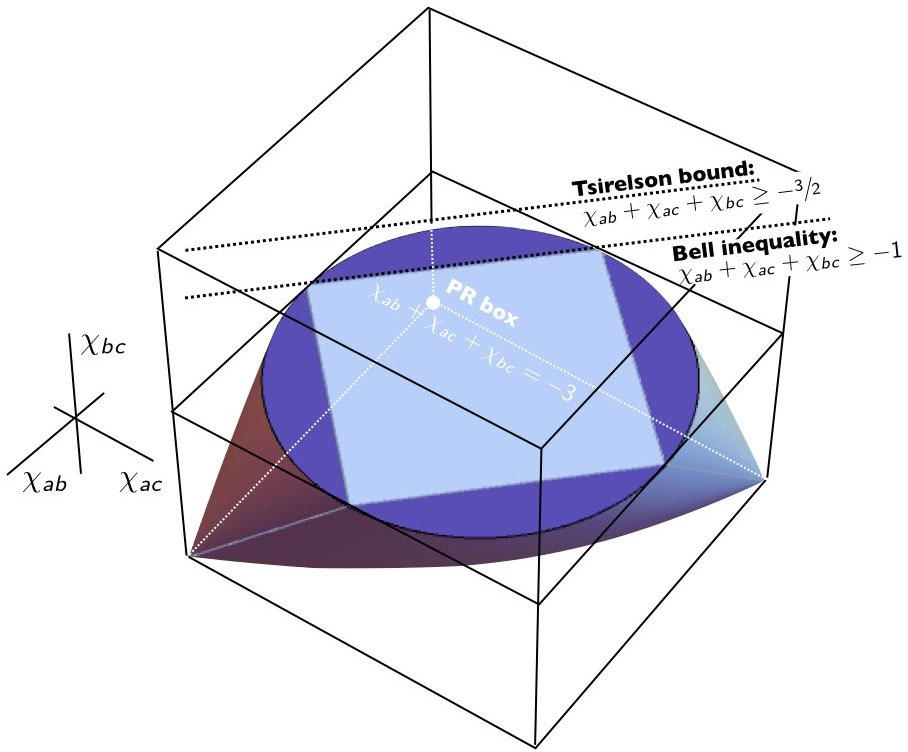
\includegraphics[width=4.6in]{elliptope-LQPslice.jpeg}
\caption{Concrete version of the diagram in Figure \ref{LQP} for the correlations in the Mermin setup. The figure shows the cross-section $\chi_{bc} =0$ of the classical tetrahedron and the elliptope in a non-signaling cube in ordinary three-dimensional space (cf.\ Figures \ref{tetrahedron} and \ref{elliptope} below). See Sections  \ref{1.4}--\ref{1.5} for discussion of the two dotted lines representing two inequalities for the sum of the anti-correlation coefficients $\chi_{ab}$, $\chi_{ac}$ and $\chi_{bc}$. These inequalities are maximally violated in the point $(-1, -1, -1)$, which thus represents the PR box for this setup.}
   \label{elliptope-LQPslice}
\end{figure} 

Figure \ref{LQP} gives a schematic representation of the non-signaling polytope for such a setup. The outer square and everything inside of it (the non-signaling polytope $\mathcal{P}$) represents the set of all non-signaling correlations. The inner square and everything inside of it (the local polytope $\mathcal{L}$) represents the set of all non-signaling correlations allowed classically (i.e., by a local hidden-variable theory). The circle in between these two squares and everything inside of it (the quantum convex set $\mathcal{Q}$) represents the set of all correlations allowed quantum-mechanically. One of the facets of $\mathcal{L}$ represents a Bell inequality, a bound on the strength of the correlations allowed classically. The vertex of the non-signaling cube where this bound is maximally violated represents a PR box for the setup under consideration.

Figure \ref{CA-3set2out-Mermin} shows the correlation array for our version of Mermin's example of a quantum correlation violating a Bell inequality. We will refer to it as the \emph{Mermin correlation array}. Its nine cells form a $3 \times 3$ grid. The cells along the diagonal of this grid, when Alice and Bob peel the same way, show a perfect anti-correlation. The six off-diagonal cells, when Alice and Bob peel differently, all show the same imperfect positive correlation. It is easy to see that this correlation array is non-signaling: the entries in both rows and both columns of all nine cells add up to $\sfrac12$. Concisely put, this correlation (array) has \emph{uniform marginals}.

The Mermin correlation array in Figure \ref{CA-3set2out-Mermin} is a special case of the more general correlation array in Figure \ref{CA-3set2out-non-signaling-chis}. The three cells along the diagonal are the same, all showing a perfect anti-correlation (i.e., its diagonal elements are 0 and its off-diagonal elements are $\sfrac12$). Moreover, cells on opposite sides of the diagonal are the same. This correlation array can thus be parametrized by three anti-correlation coefficients of the kind introduced in Figure \ref{CA-2set2out-cell} and Eq.\ (\ref{chi as corr coef}).  In the specific example of the Mermin setup in Figure \ref{CA-3set2out-Mermin}, the three anti-correlation coefficients have the same value:  
\begin{equation}
\chi_{ab} = \chi_{ac} = \chi_{bc} = -\sfrac12.
\label{chi values Mermin example}
\end{equation}

The class of all non-signaling correlations in the Mermin setup can be visualized as a cube in ordinary three-dimensional space with the correlation coefficients, $\chi_{ab}$, $\chi_{ac}$ and $\chi_{bc}$, providing the three Cartesian coordinates of points in this cube. The non-signaling correlations allowed classically can be represented by a tetrahedron spanned by four of the eight vertices of this non-signaling cube (see Figure \ref{tetrahedron} in Section \ref{1.4}); those allowed quantum-mechanically by an elliptope enclosing this tetrahedron (see Figure \ref{elliptope} in Section \ref{1.5}). Figure \ref{elliptope-LQPslice} shows the cross-section $\chi_{bc} =0$ of this non-signaling cube, the classical tetrahedron and the elliptope. This cross-section has exactly the form of the cartoonish rendering in Figure \ref{LQP} of the Vitruvian-man-like structure of the local polytope $\mathcal{L}$ and the quantum convex set $\mathcal{Q}$ inside the non-signaling polytope $\mathcal{P}$. In the next two subsections, we will show in detail how one arrives at the classical tetrahedron and the quantum elliptope in the Mermin setup.

%SUBSECTION 2.4
\subsection{Classical polytopes and raffles to simulate quantum correlations} \label{1.4}

As \citet[p.\ 10]{Bub 2016} explains in the opening chapter of \emph{Bananaworld}, to decide whether or not some correlation array is allowed classically (or quantum-mechanically), he checks whether or not it can be simulated with classical (or quantum-mechanical) resources. Though we will use a more direct approach to find classes of correlations allowed quantum-mechanically (see Sections  \ref{1.5} and \ref{2.1}), we will adopt a variation on Bub's imitation game to find classes of correlations allowed classically (i.e., by some local hidden-variable theory). 

We will use special raffles to simulate the correlations found in our quantum banana peeling and tasting experiments. These raffles involve baskets of tickets such as the ones in Figure \ref{raffle-tickets-3set2out-i-thru-iv}. All tickets list the outcomes for both parties and for all settings in the setup under consideration. We randomly draw a ticket of the appropriate kind from a basket with many such tickets. We tear this ticket in half and randomly decide which side goes to Alice and which side goes to Bob. Alice and Bob then decide, randomly and independently of each other, which setting they will use. They record the outcome for that setting printed on their half of the ticket. We repeat this procedure a great many times. 

Raffles of this kind provide a criterion for determining whether or not a certain correlation is allowed classically:\footnote{In Section \ref{4} we will see that there is an extra bonus to discussing classical theory in terms of such raffles. It makes for a natural comparison between local hidden-variable theories and John von Neumann's (1927b) formulation of quantum theory in terms of statistical ensembles characterized by density operators on Hilbert space. \emph{Single-ticket raffles}, i.e., raffles with baskets of tickets that are all the same, are the classical analogues of pure states in quantum mechanics; \emph{mixed raffles}, i.e., raffles with baskets with different tickets, are the analogues of mixed states. By using the imagery of baskets with different mixes of tickets, we admittedly sweep a mathematical subtlety under the rug: the fractions of different types of tickets in a basket will always be rational numbers. To simulate the quantum correlations we are interested in, however, we need to allow fractions that are real numbers. In Section \ref{2.2.1} we will introduce a different mechanism for selecting tickets that gets around this problem (see Figure \ref{wheelsoffortune}). From a practical point of view, the restriction to rationals is harmless, since the rationals are dense in the reals.\label{dense}}
\begin{quote}
\emph{A correlation array is allowed by a local hidden-variable theory if and only if there is a raffle (i.e., a basket with the appropriate mix of tickets) with which we can simulate that correlation array following the protocol described above.}
\end{quote}

\begin{figure}[ht]
 \centering
   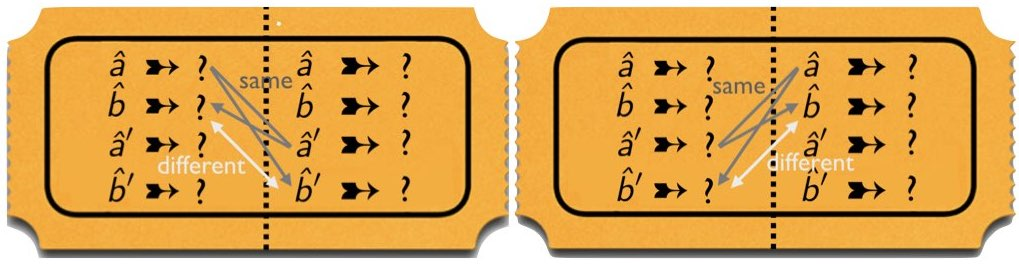
\includegraphics[width=4.5in]{raffle-ticket-PRbox.jpeg} 
   \caption{Trying to design a raffle ticket for a PR box.}
   \label{raffle-ticket-PRbox}
\end{figure}

Invoking this criterion, we can easily show that a PR box with the correlation array in Figure \ref{CA-PRbox} is not allowed classically.\footnote{Essentially the same argument can already be found in \citet[p.\ 970]{Rastall 1995}.} These correlations place impossible demands on the design of the tickets for a raffle that would simulate them (see Figure \ref{raffle-ticket-PRbox}). The perfect positive correlation between the outcomes for three of the four possible combinations of settings ($\hat{a} \, \hat{a}'$, $\hat{a} \, \hat{b}'$ and $\hat{b} \, \hat{a}'$) requires that the outcomes printed on the ticket for $\hat{a}$ and $\hat{b}$ on one side are the same as the outcomes for $\hat{a}'$ and $\hat{b}'$ on the other side. That makes it impossible for the outcomes for $\hat{b}$ and $\hat{b}'$ on opposite sides of the ticket to be different as required by the perfect anti-correlation for the remaining combination of settings ($\hat{b} \, \hat{b}'$). 

\begin{figure}[ht]
 \centering
   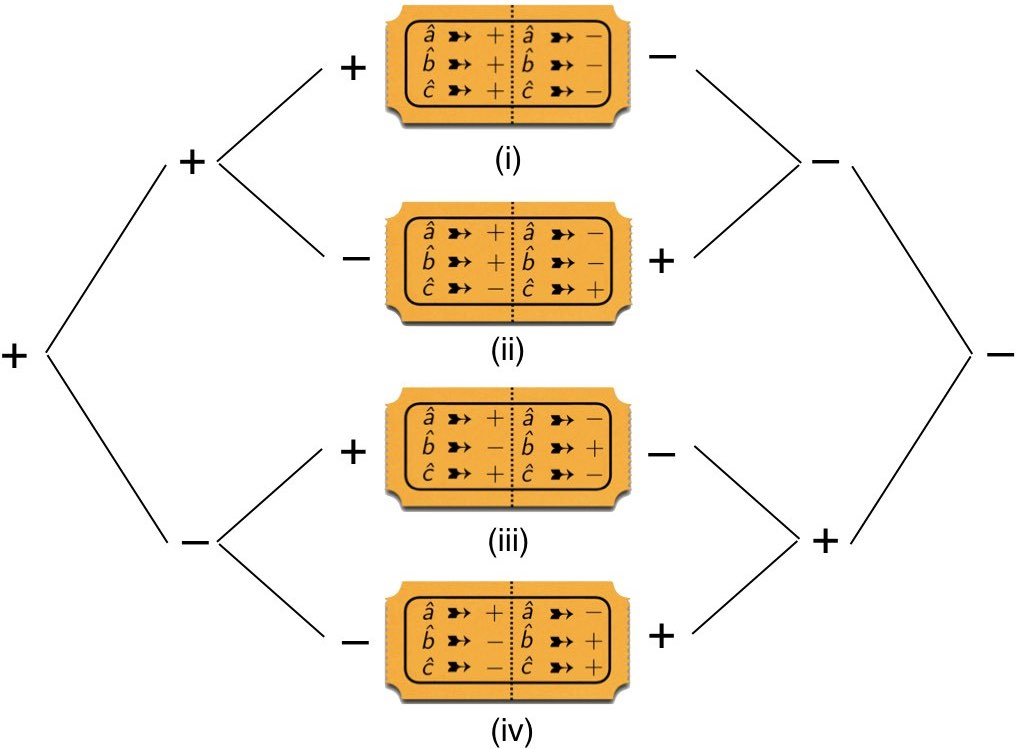
\includegraphics[width=4.5in]{raffle-tickets-3set2out-i-thru-iv.jpeg} 
   \caption{The four different raffle tickets for three settings and two outcomes. Given the protocol of our raffles, two tickets that differ only in that their left and right sides are swapped are the same ticket.}
   \label{raffle-tickets-3set2out-i-thru-iv}
   \end{figure}

Figure \ref{raffle-tickets-3set2out-i-thru-iv} shows four different types of tickets, labeled (i) through (iv), for raffles meant to simulate correlations found in the Mermin setup in which Alice and Bob choose from the same three settings $(\hat{a}, \hat{b}, \hat{c})$ with two possible outcomes each $(+, -)$. Since in all setups that we will examine Alice and Bob find opposite results whenever they use the same setting, the outcomes on one side of the ticket dictate the outcomes on the other. That reduces the number of different ticket types to $2^3 = 8$. Given that it is decided randomly which side of a ticket goes to Alice and which side to Bob, two tickets that differ only in that the left and the right side are swapped are two equivalent versions of the same ticket type. This further reduces the number of different ticket types to four. As illustrated in Figure \ref{raffle-tickets-3set2out-i-thru-iv}, we chose the ones that have $+$ for the first setting ($\hat{a}$) on the left side of the ticket.


\begin{figure}[ht]   
 \centering
   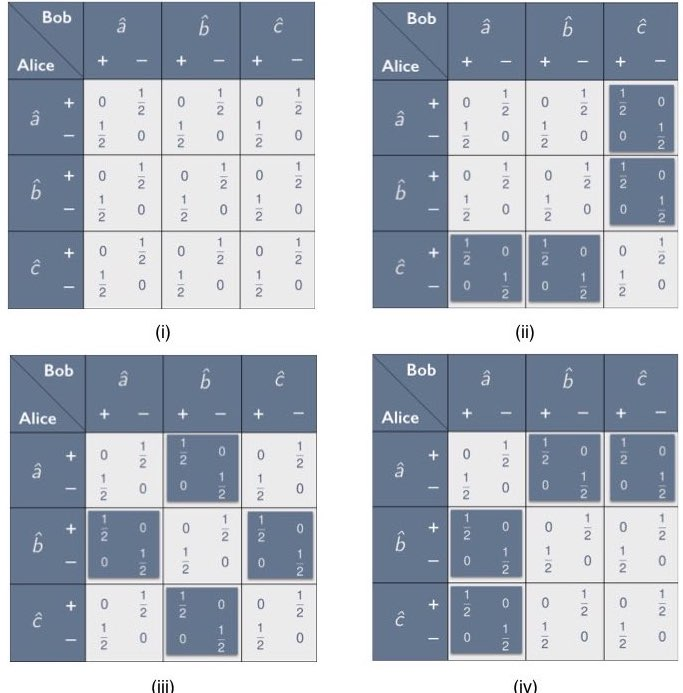
\includegraphics[width=4.5in]{CA-3set2out-raffles-i-thru-iv.jpeg} 
   \caption{Correlation arrays for raffles for the four different single-ticket raffles in the Mermin setup. In blue-on-white cells the outcomes are perfectly anti-correlated; in white-on-blue cells they are perfectly correlated.}
   \label{CA-3set2out-raffles-i-thru-iv}
\end{figure}

Figure \ref{CA-3set2out-raffles-i-thru-iv} shows the correlation arrays for raffles with baskets containing only one of the four types of tickets in Figure \ref{raffle-tickets-3set2out-i-thru-iv}. The design of our raffles guarantees that the correlations between the outcomes found by Alice and Bob are non-signaling. This is borne out by the correlation arrays in Figure \ref{CA-3set2out-raffles-i-thru-iv}. The entries in both rows and both columns of all cells in these correlation arrays add up to $\sfrac12$. In other words, these raffles all give uniform marginals. The design of our raffle tickets also guarantees that the outcomes found by Alice and Bob are \emph{balanced} (see the definition in the sentence following  Eq.\ (\ref{cov def 0})).

The entries of correlation arrays like those in Figure \ref{CA-3set2out-raffles-i-thru-iv} form $6 \times 6$ matrices. These matrices are symmetric. This is true both for single-ticket and mixed raffles. All raffles we will consider have this property. This too follows directly from the design of these raffles. It is simply because Alice and Bob are as likely to get the left or the right side of any ticket. 

\begin{figure}[ht]   
 \centering
   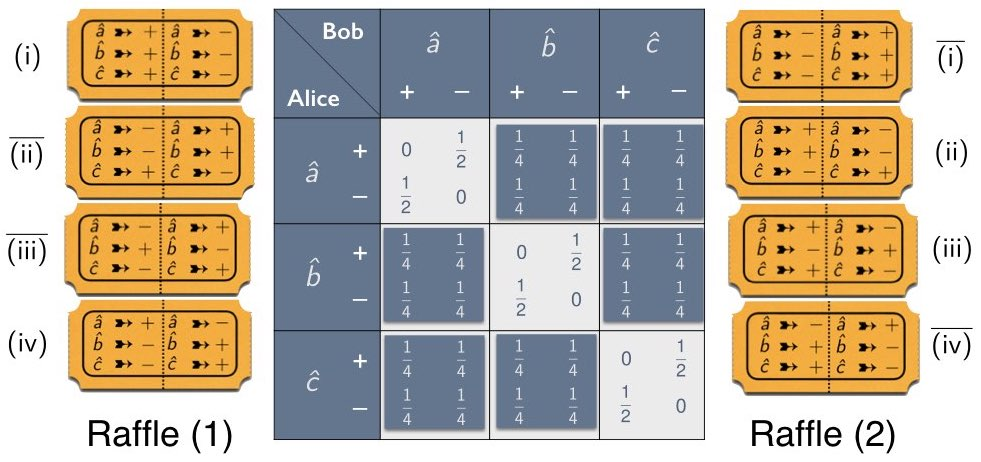
\includegraphics[width=4.5in]{CA-3set2out-raffle-25i25ii25iii25iv.jpeg} 
   \caption{Two raffles leading to the same correlation array (in blue-on-white cells the outcomes are perfectly anti-correlated; in white-on-blue cells they are completely uncorrelated). In both raffles, whenever a ticket is drawn, Alice gets the left and Bob gets the right side. In addition to tickets (i)--(iv) in Figure \ref{raffle-tickets-3set2out-i-thru-iv} we now have four more tickets, labeled $\overline{(\mathrm{i})}$-$\overline{(\mathrm{iv})}$ and obtained by switching the left and the right side of the tickets (i)--(iv).  Raffle (1) has equal numbers of tickets of type (i), $\overline{(\mathrm{ii})}$, $\overline{(\mathrm{iii})}$ and (iv). Raffle (2) has equal numbers of tickets of type $\overline{(\mathrm{i})}$, (ii), (iii) and $\overline{(\mathrm{iv})}$.}
   \label{CA-3set2out-raffle-25i25ii25iii25iv}
\end{figure}

Before we continue our analysis, we show that changing the protocol of our raffles so that Alice is always given the left side and Bob is always given the right side of any ticket does not give rise to correlation arrays with symmetric associated matrices that cannot be simulated with our more economical protocol---more economical because it requires fewer ticket types. For the alternative protocol, we need four more tickets, labeled $\overline{(\mathrm{i})}$ through $\overline{(\mathrm{iv})}$, that differ from their counterparts (i) through (iv) in that the left and right sides of the ticket have been swapped. Figure \ref{CA-3set2out-raffle-25i25ii25iii25iv} shows two raffles for this alternative protocol. Raffle (1) has equal numbers of tickets of type $\big\{ \mathrm{(i)}, \overline{(\mathrm{ii})}, \overline{(\mathrm{iii})}, \mathrm{(iv)} \big\}$. The matrix associated with the correlation array for this raffle is symmetric. That means that we get the same correlation array if we swap the left and the right sides of all tickets in raffle (1). This turns raffle (1) into raffle (2) with equal numbers of tickets of type $\big\{ \overline{(\mathrm{i})}, \mathrm{(ii)}, \mathrm{(iii)}, \overline{(\mathrm{iv})} \big\}$.  Any raffle mixing raffles (1) and (2) will also give that same correlation array. Consider the special case of a raffle with equal numbers of all eight tickets. This raffle is equivalent to a basket with equal numbers of tickets $\big\{  \mathrm{(i)},  \mathrm{(ii)},  \mathrm{(iii)},  \mathrm{(iv)} \big\}$ with the understanding that it is decided at random which side of the ticket goes to Alice and which side goes to Bob. This construction works for any correlation array with a symmetric associated matrix that we can produce using the protocol in which Alice always get the left side and Bob always get the right side of a ticket. We conclude that we can produce any such correlation array using our more economical protocol. 

\begin{figure}[ht]
 \centering
   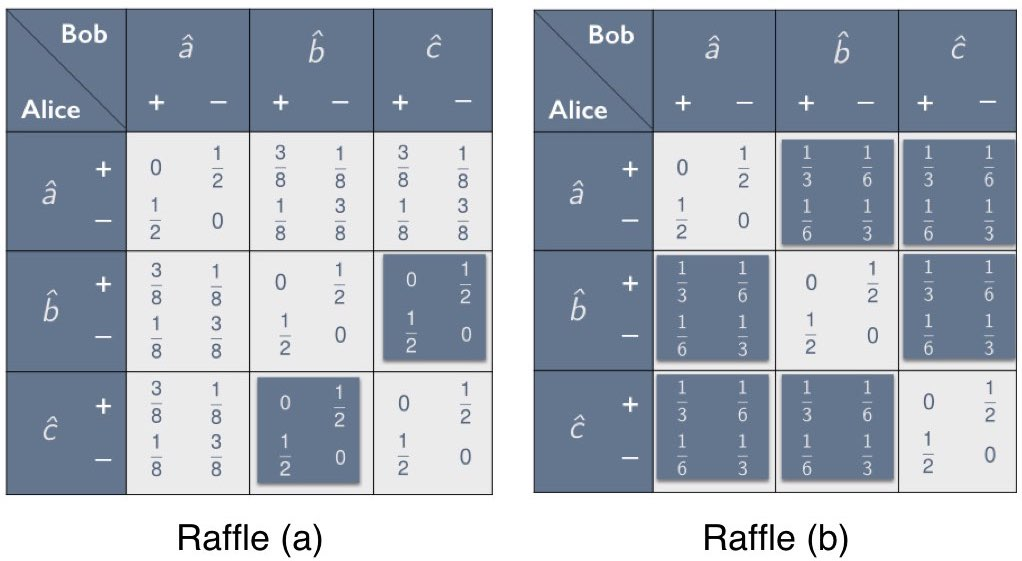
\includegraphics[width=4.5in]{CA-3set2out-raffle-mix.jpeg} 
   \caption{Correlation arrays for raffles with different mixes of the four tickets in Figure \ref{raffle-tickets-3set2out-i-thru-iv}. Raffle (a) has 25\%  type-(i) tickets and 75\% type-(iv) tickets. Raffle (b) has 33\% each of type-(ii) through type-(iv) tickets. Blue-on-white cells are the same as the corresponding cells in the Mermin correlation array in Figure \ref{CA-3set2out-Mermin}, white-on-blue cells are different.}
   \label{CA-3set2out-raffle-mix}
\end{figure}

There is no mix of tickets (i) through (iv) in Figure \ref{raffle-tickets-3set2out-i-thru-iv} that produces a raffle that can simulate the Mermin correlation array in Figure \ref{CA-3set2out-Mermin}. Figure \ref{CA-3set2out-raffle-mix} shows the results of two unsuccessful attempts to produce one. In the first, we take a basket with 25\% tickets of type (i) and 75\% of type (iv). This results in correlation array (a) in Figure \ref{CA-3set2out-raffle-mix}. This raffle correctly simulates all but two cells of the Mermin correlation array. We get the same result if we replace tickets (iv) by tickets (ii) or (iii), the only difference being that now two other cells will differ from the corresponding ones in the Mermin correlation array. The best we can do overall is to take a basket with 33\% each of tickets (ii) through (iv). This results in correlation array (b) in Figure \ref{CA-3set2out-raffle-mix}. Like the Mermin correlation array we are trying to simulate, this one has the same positive correlation in all six off-diagonal cells but the correlation is weaker ($-\chi_{ab} = -\chi_{ac} = -\chi_{bc}  = \sfrac13$) than in the Mermin case ($-\chi_{ab} =-\chi_{ac}  = -\chi_{bc}  = \sfrac12$).

To prove that there is no raffle that can simulate the Mermin correlation array, we consider the sum $\chi_{ab} + \chi_{ac} + \chi_{bc}$ of the anti-correlation coefficients for a raffle. From the tickets in Figure \ref{raffle-tickets-3set2out-i-thru-iv} we can read off the values of $\chi_{ab}$, $\chi_{ac}$ and $\chi_{bc}$ for the four single-ticket raffles. These values are brought together in Table \ref{values of chi}. 

\begin{table}[ht]
\centering
\begin{tabular}{|c||c|c|c|}
\hline
ticket & \quad $\chi_{ab}$ \quad & \quad $\chi_{ac}$ \quad & \quad $\chi_{bc}$ \quad \\[.1cm] 
\hline
 (i) & $+1$ & $+1$ & $+1$ \\[.2cm]
 (ii) & $+1$ & $-1$ & $-1$ \\[.2cm]
 (iii) & $-1$ & $+1$ & $-1$ \\[.2cm]
(iv) & $-1$ & $-1$ & $+1$ \\
 \hline
\end{tabular}
\caption{Values of the anti-correlation coefficients parametrizing the off-diagonal cells of the correlation arrays (i) through (iv) in Figure \ref{CA-3set2out-raffles-i-thru-iv} for single-ticket raffles with tickets (i) through (iv) in Figure \ref{raffle-tickets-3set2out-i-thru-iv}.}
\label{values of chi}
\end{table} 

The cells in the correlation arrays in Figure \ref{CA-3set2out-raffles-i-thru-iv} are all either perfectly anti-correlated or perfectly correlated. The anti-correlation coefficients for these single-ticket raffles can therefore only take on the values $\pm 1$ and their sum can only take on the value 3 (for a raffle with tickets of type (i) only) or $-1$ (for raffles with tickets (ii) or (iii) or (iv) only). For mixed raffles, $\chi_{ab} + \chi_{ac} + \chi_{bc}$ is the weighted average of the value of $\chi_{ab} + \chi_{ac} + \chi_{bc}$ for these four single-ticket raffles, with the weights given by the fractions of each of the four tickets in the raffle.\footnote{For a formal proof of this intuitively plausible result, see Section \ref{2.2.1}.} Hence, for any mix of tickets, this sum must lie between $-1$ and $3$:
\begin{equation}
-1 \le \chi_{ab} + \chi_{ac} + \chi_{bc} \le 3.
\label{Mermin inequality CHSH-like}
\end{equation}
The first of these inequalities, giving the lower bound on $\chi_{ab} + \chi_{ac} + \chi_{bc}$, is the analogue of the CHSH inequality for our variation of the Mermin setup. It is also the form in which \citet{Bell 1964} originally derived the Bell inequality. The CHSH-type Bell inequality is violated by the Mermin correlation array in Figure \ref{CA-3set2out-Mermin}. In that case, $\chi_{ab} = \chi_{ac} = \chi_{bc} = - \sfrac12$ (see Eq.\ (\ref{chi values Mermin example})) and their sum equals $-\sfrac32$. As we will see in Section \ref{1.5}, this is the maximum violation of this inequality allowed by quantum mechanics. Note that the absolute minimum value of $\chi_{ab} + \chi_{ac} + \chi_{bc}$ is $-3$. This value is allowed neither classically nor quantum-mechanically. It is the value reached with the (hypothetical) PR box for this setup.  

\begin{figure}[ht]
 \centering
   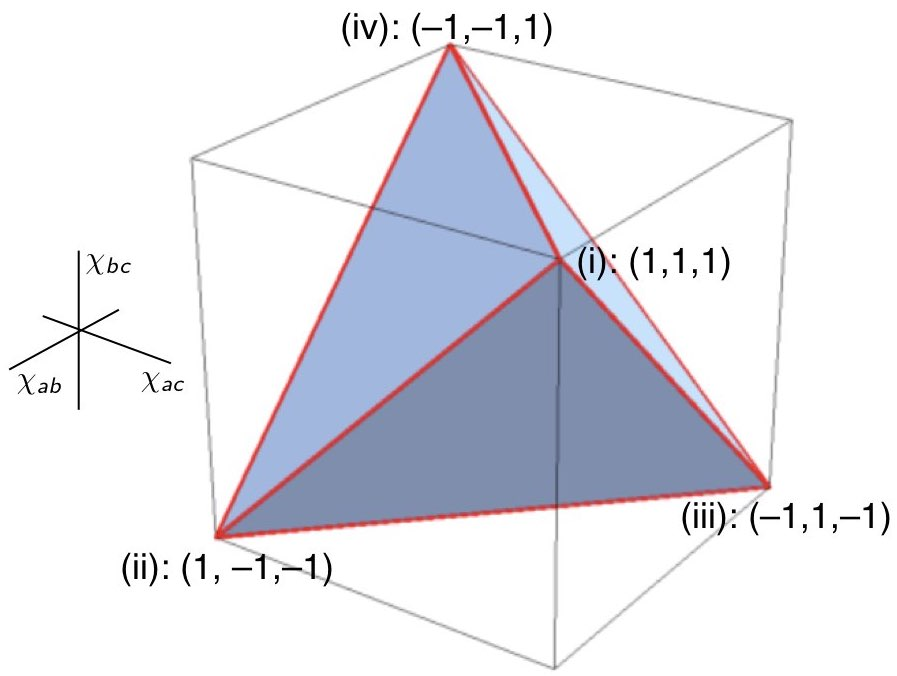
\includegraphics[width=4.5in]{tetrahedron.jpeg} 
   \caption{Tetrahedron of triplets of anti-correlation coeffcients $(\chi_{ab}, \chi_{ac}, \chi_{bc})$ allowed by local hidden-variable theories in our version of the Mermin setup.}
   \label{tetrahedron}
\end{figure}

The values of $\chi_{ab}$,  $\chi_{ac}$ and $\chi_{bc}$ in Table \ref{values of chi} for tickets (i) through (iv) can be used as the Cartesian coordinates of four vertices in the non-signaling cube for the Mermin setup. These are the vertices labeled (i) through (iv) in Figure \ref{tetrahedron}. The vertex $(-1, -1, -1)$ represents the PR box for this setup (see Figure \ref{elliptope-LQPslice}). The vertices (i) through (iv) span a tetrahedron forming the convex set of all raffles that can be obtained by mixing the four types of tickets. The sum $\chi_{ab} + \chi_{ac} + \chi_{bc}$ takes on its maximum value of 3 at the vertex for tickets of type (i) and its minimum value of $-1$ for the facet spanned by the vertices for tickets of types (ii), (iii) and (iv). The inequalities in Eq.\ (\ref{Mermin inequality CHSH-like}) tell us that all correlations that can be simulated with raffles with various mixes of tickets must lie in the region of the non-signaling cube between the vertex (i) and the facet (ii)-(iii)-(iv). 

This is a necessary but not a sufficient condition for a correlation to be allowed by a local hidden-variable theory. As Figure \ref{tetrahedron} shows, there are three forbidden sub-regions in the region between vertex (i) and facet (ii)-(iii)-(iv). A full characterization of the class of correlations allowed classically requires three additional pairs of inequalities like the pair given in Eq.\ (\ref{Mermin inequality CHSH-like}), corresponding to the other three vertices and the other three facets of the tetrahedron. The following four pairs of inequalities do fully characterize the tetrahedron:
\begin{eqnarray}
-1 \le \;\, \chi_{ab} + \chi_{ac} + \chi_{bc} \; \le 3  & \!\!\!\! & \textrm{[between facet (ii)-(iii)-(iv) and vertex (i)]} 
\label{Mermin inequality CHSH-like (i)} \\[.4cm]
-1 \le \;\, \chi_{ab} - \chi_{ac} - \chi_{bc} \; \le 3  & \!\!\!\!  & \textrm{[between facet (i)-(iii)-(iv) and vertex (ii)]}  
\label{Mermin inequality CHSH-like (ii)} \\[.4cm]
-1 \le - \chi_{ab} + \chi_{ac} - \chi_{bc} \le 3 & \!\!\!\!  & \textrm{[between facet (i)-(ii)-(iv) and vertex (iii)]} 
\label{Mermin inequality CHSH-like (iii)} \\[.4cm]
-1 \le - \chi_{ab} - \chi_{ac} + \chi_{bc} \le 3 & \!\!\!\!   & \textrm{[between facet (i)-(ii)-(iii) and vertex (iv)]}.
\label{Mermin inequality CHSH-like (iv)}
\end{eqnarray}
Using the symmetries of the tetrahedron we can easily get from any one of these pairs of inequalities to another.  Another way to see this is to recall that the coordinates $(\chi_{ab}, \chi_{ac}, \chi_{bc})$ are anti-correlation coefficients for different combinations of the measurement settings $(\hat{a}, \hat{b}, \hat{c})$ and to look at what happens when we flip the sign of the outcomes for one of these three settings. If we do this for $\hat{a}$, $\chi_{ab}$ and $\chi_{ac}$ pick up a minus sign and Eq.\ (\ref{Mermin inequality CHSH-like (i)}) turns into Eq.\ (\ref{Mermin inequality CHSH-like (iv)}). If we do this for $\hat{b}$, $\chi_{ab}$ and $\chi_{bc}$ pick up a minus sign and Eq.\ (\ref{Mermin inequality CHSH-like (i)}) turns into Eq.\ (\ref{Mermin inequality CHSH-like (iii)}). Finally, if we do this for $\hat{c}$, $\chi_{ac}$ and $\chi_{bc}$ pick up a minus sign and Eq.\ (\ref{Mermin inequality CHSH-like (i)}) turns into Eq.\ (\ref{Mermin inequality CHSH-like (ii)}).

Mermin formulated a different inequality for this setup, one that implies the lower bound on the sum of anti-correlation coefficients in Eq.\ (\ref{Mermin inequality CHSH-like}) but requires an additional assumption. To derive Mermin's inequality, we have to assume that \emph{Alice and Bob randomly and independently of each other decide which setting to use in any run of the experiment} (whether with raffle tickets, spin-$\frac12$ particles, or quantum bananas). This provision is part of the protocol we described in Section \ref{1.1} but we had no need to invoke it so far. The CHSH-like inequality in Eq.\ (\ref{Mermin inequality CHSH-like}) could be derived without it---and so, for that matter, can the CHSH inequality itself. 

This means that we can test these inequalities without having to change the settings in every run. We can make measurements for one pair of settings at a time, providing data for the correlation array one cell at a time. This is how \citet{Clauser and Freedman 1972} originally tested the CHSH inequality. Changing the orientation of their polarizers was a cumbersome process.\footnote{For a drawing of their apparatus see \citet[p.\ 262]{Gilder 2008}. This drawing is based on a photograph that can be found, for instance, in \citet[p.\ 48]{Kaiser 2011}. For a schematic drawing of the apparatus, see  \citet[p.\ 939, Figure 1]{Clauser and Freedman 1972}.} Because of this limitation of their equipment, the violation of the CHSH inequality they found could conceivably be blamed on the two photons generated as an entangled pair ``knowing'' ahead of time (i.e., the moment they separated) what the orientation of the polarizers would be with which they were going to be measured. To close this loophole, the settings should only be chosen once the photons are in flight. This was accomplished by Aspect and his collaborators later in the 1970s and in the 1980s \citep[Ch.\ 31]{Gilder 2008}. In this paper, we will not be concerned with the extensive experimental efforts to close this and other loopholes.\footnote{David Kaiser alerted us to a paper written by 20 authors (with Kaiser, Alan Guth and Anton Zeilinger listed in 17th, 18th and 20th place, respectively) about one of the latest initiatives in this ongoing effort \citep{Handsteiner 2017}.} 

If we assume that Alice and Bob randomly and independently of each other decide which setting to use in each run,\footnote{We still do not need the stronger assumption that these decisions are made only after they receive their banana, their spin-$\frac12$ particle, or their ticket stub.} the nine possible combinations of settings are equiprobable. Following \citet[pp.\ 86--87]{Mermin 1981}, we ask for the probability, $\mathrm{Pr(opp)}$, that Alice and Bob find opposite results. Consider the Mermin correlation array in Figure \ref{CA-3set2out-Mermin}. For the cells along the diagonal $\mathrm{Pr(opp)} = 1$ (the results are perfectly anti-correlated). For the off-diagonal cells $\mathrm{Pr(opp)} = \sfrac14$, the sum of the off-diagonal entries in those cells. Alice and Bob use the same setting in one out of three runs and different settings in two out of three. Hence, the probability of them finding opposite results is:
\begin{equation}
\mathrm{Pr(opp)} = \sfrac13 \cdot 1 \, + \, \sfrac23 \cdot \sfrac14 = \sfrac12.
\label{Pr opp Mermin}
\end{equation}
Upon inspection of the four correlation arrays in Figure \ref{CA-3set2out-raffles-i-thru-iv}, however, we see that the minimum value for $\mathrm{Pr(opp)}$ in a local hidden variable theory is $\sfrac59$. In correlation array (i), the results in all nine cells are perfectly anti-correlated. In a single-ticket raffle with tickets of type (i), we thus have $\mathrm{Pr(opp)} = 1$.  In each of the other three correlation arrays, there are five cells in which the results are perfectly anti-correlated and four in which they are perfectly correlated. In single-ticket raffles with tickets of type (ii), (iii), or (iv), we thus have $\mathrm{Pr(opp)} = \sfrac59$. For an arbitrary mix of tickets (i) through (iv), we therefore have the inequality
\begin{equation}
\mathrm{Pr(opp)} \ge \sfrac59.
\label{Mermin inequality probs}
\end{equation}
This is the form in which Mermin states the Bell inequality for the setup we are considering. It implies the lower bound in Eq.\ (\ref{Mermin inequality CHSH-like}). Consider, once again, the general non-signaling correlation array in Figure \ref{CA-3set2out-non-signaling-chis} parametrized by the anti-correlation coefficients $\chi_{ab}$, $\chi_{ac}$ and  $\chi_{bc}$. Adding the off-diagonal elements in every cell and dividing by 9, as we are assuming that Alice and Bob use the settings of all nine cells with equal probability, we find
\begin{eqnarray}
\mathrm{Pr(opp)} & \!\! = \!\! & \sfrac39 \, + \, \sfrac29 \cdot \sfrac12 \, \Big(1+ \chi_{ab} \Big) \, + \, \sfrac29 \cdot \sfrac12 \, \Big(1+ \chi_{ac} \Big) \, + \,  \sfrac29 \cdot \sfrac12 \, \Big(1+ \chi_{bc} \Big) \nonumber \\[.2cm]
 & \!\! = \!\!  & \sfrac{2}{3} \, + \, \sfrac{1}{9} \, \Big(\chi_{ab} + \chi_{ac} + \chi_{bc} \Big). 
 \label{Pr opp general} 
\end{eqnarray}
If $\mathrm{Pr(opp)}$ must at least be $\sfrac59$, then $\chi_{ab} + \chi_{ac} + \chi_{bc}$ cannot be smaller than $-1$. Conversely, if $\chi_{ab} + \chi_{ac} + \chi_{bc} \ge -1$ \emph{and} all nine combinations of the settings $\hat{a}$, $\hat{b}$ and $\hat{c}$ are equiprobable, then 
$\mathrm{Pr(opp)} \ge \sfrac59$. 
 
Mermin's lower bound on the probability of finding opposite results may be easier to grasp for a general audience than a lower bound on a sum of expectation values. The latter, however, does have its own advantages. First, as we just saw, it can be derived from weaker premises. Second, it immediately generates inequalities corresponding to other facets of the polyhedron of classically allowed correlations in the Mermin setup (see Eqs. (\ref{Mermin inequality CHSH-like (i)})--(\ref{Mermin inequality CHSH-like (iv)})). Third, as we will show in detail in Section \ref{3}, it makes it easier to see the connection with the CHSH inequality.

